\chapter{Wireless M-Bus protokol}
Wireless M-Bus je v Evropě perspektivní otevřený standard pro automatické měření, který pracuje v subgi-gaherzovém bezlicenčním pásmu v okolí 868 MHz. Wireless M-Bus se primárně zaměřuje na použití v SRD (Short Range Device) zařízeních pro bezdrátovou komunikaci s měřiči energií, jako jsou: voda, plyn, teplo, elektřina, atd. Měřiče energií, vybavené bezdrátovým rozhraním Wireless M-Bus jsou schopny komunikovat jak se stacionárními, tak i s mobilními čtecími zařízeními. Předpokládá se, že rádiová část měřiče je napájena z baterie a je schopna provozu po dlouhou dobu bez zásahu, tj. bez výměny baterie. Na čtecích zařízeních, ať už stacionárních nebo mobilních, není takový požadavek na dobu provozu na baterie a čtecí zařízení mohou být napájena i z externího zdroje.

Wireless M-Bus má svůj původ v rámci norem Meter-Bus. Wireless Meter Bus je~bezdrátovou variantou drátového Meter-Bus. To je standard zaměřený na aplikace pro sběr dat měřiče plynu, elektřiny a vody. Sběrnice je specifikována v evropské normě EN 13757~\cite{Norma1}. Tato specifikace je rozdělena do pěti částí (viz Tab.~\ref{TableNorma}), z~nichž jedna se zaměřuje na Wireless M-Bus.

\begin{table}[!ht]
\centering
\caption{Popis standardu EN-13757~\cite{WmbusTables}}
\label{TableNorma}
\resizebox{\textwidth}{!}{%
\begin{tabular}{|l|l|}
\hline
{\textbf{Standard}} & \multicolumn{1}{c|}{\textbf{Podrobnosti}} \\ \hline \hline
EN 13757-1 & \begin{tabular}[c]{@{}l@{}}Část 1 standardu definuje výměnu dat, která podrobně popisuje základní \\ komunikaci mezi vodoměry a centrálním sběračem dat. Poskytuje přehled \\ komunikačního systému.\end{tabular}\\ \hline
EN 13757-2 & \begin{tabular}[c]{@{}l@{}}Tato část normy Meter Bus řeší fyzickou a spojovou vrstvu pro fyzický přenos \\ dat pomocí kabelových spojů. Také popisuje protokol používaný pro přenos dat\end{tabular} \\ \hline
EN 13757-3 & \begin{tabular}[c]{@{}l@{}}Část 3  se týká speciální aplikační vrstvy. Ta popisuje standardní aplikační\\  protokol používaný k tomu, aby se zachovala kompatibilita výrobců, což \\ umožňuje zařízení od několika různých dodavatelů působit v jednom systému.\end{tabular} \\ \hline
EN 13757-4 & \begin{tabular}[c]{@{}l@{}}Oddíl 4 popisuje bezdrátový systém. Jedná se o radiový odečet pro provoz v pásmu \\ 868 MHz až 870 MHz . Tato část normy se zabývá fyzickou a linkovou vrstvou pro\\  bezdrátová zařízení.\end{tabular} \\ \hline
EN 13757-5 & \begin{tabular}[c]{@{}l@{}}Tato část definuje adresy předávání. To zahrnuje celou řadu návrhů na předávání \\ datových rámců jako prostředek komunikace mezi měřičem a koncentrátorem.\end{tabular} \\ \hline \hline
\end{tabular}}
\vspace{-10pt}
\end{table}

%%%%%%%%%%%%%%%%%%%%%%%%%%%%%%%%%%%%%%%%%%%%%%%%%=
%%%%%%%%%%%%%%%%%%%%%%%%%%%%%%%%%%%%%%%%%%%%%%%%%=
%%%%%%%%%%%%%%%%%%%%%%%%%%%%%%%%%%%%%%%%%%%%%%%%%=
%%%%%%%%%%%%%%%%%%%%%%%%%%%%%%%%%%%%%%%%%%%%%%%%%=

\section{Princip komunikace}

Bezdrátová komunikace Wireless M-Bus fyzicky probíhá ve 12 kanálech v bezplatném vysílacím pásmu ISM (industrial, scientific and medical) okolo frekvence 868\,MHz (2~kanály\,868,3 a 868,95\,MHz jsou využívány režimem S a T, 10 uživatelem volitelných kanálů 868.03 + n x 0.06\,MHz v režimu R2), přičemž každý z výše uvedených režimů vyžaduje různé požadavky. Těmi například jsou specifikovaný kanál, přesnost frekvence, toleranci přenosové rychlosti atd. Velmi dobrá je stabilita frekvence až 27 let (dle údaje výrobce). V případě použití čtvrtvlné antény (délky 8,2 cm), tak na přímou viditelnost vysílací a přijímacího modulu je komunikační dosah 500 až 600\,m.

Komunikace má hvězdicovitou strukturu, kdy několik měřících jednotek/snímačů přenáší svá naměřená data jedné centrální jednotce, obvykle tvořené koncentrátorem. Ten tedy obvykle slouží pro příjem a shromaždování dat z několika měřících míst, z dále uvedených důvodů nikdy neinicializuje (nezahajuje) vzájemnou komunikaci. Pracuje tedy jako server (Master), tzn. že stále naslouchá a čeká na navázání komunikace měřící jednotkou a jí inicializovaný přenos dat. Ta tedy pracuje jako klient (Slave). V případě nastavené obousměrné komunikace přechází měřič/snímač do přijímacího režimu pouze po krátký čas jím navázané komunikace. Pouze v tomto momentu může koncentrátor vyslat nějaké jednotce řídící data. Časování je rozdílné pro různé režimy a je přesně specifikováno ve standardu.

Adresování ve Wireless M-Bus sběrnici je převzato z klasické drátové verze M-BUSu. Zde však pouze klientské jednotky (měřiče/snímače) mají přidělenou adresu a využívají ji jak při příjmu, tak při vysílání. Každý koncentrátor by měl obsahovat tabulku adres, se kterými může komunikovat, resp. od kterých má přijímat data. Tato tabulka se obvykle vytváří automaticky během instalace/registrování nové jednotky do sítě. Samozřejmě je možné se obejít i bez ní, ale pak lze přijímat všechny snímače či měřiče v dosahu. Toho se dá využít jen v malých sítích. 

%%%%%%%%%%%%%%%%%%%%%%%%%%%%%%%%%%%%%%%%%%%%%%%%%=
%%%%%%%%%%%%%%%%%%%%%%%%%%%%%%%%%%%%%%%%%%%%%%%%%=
%%%%%%%%%%%%%%%%%%%%%%%%%%%%%%%%%%%%%%%%%%%%%%%%%=
%%%%%%%%%%%%%%%%%%%%%%%%%%%%%%%%%%%%%%%%%%%%%%%%%=

\section{Režimy přenosu}
Nejdůležitější vlastností technologie WM-Bus je možnost bateriového napájení měřicích zařízení. V případě bezdrátové komunikace je výhodné například měřiče tepla nebo vodoměry napájet jen bateriově a tím eliminovat jakoukoliv nutnost pokládání kabelů. To ale znamená velmi omezenou spotřebu elektrické energie, aby baterie vydržely co nejdéle, alespoň několik let. V současné době v případě napájení modulu lze dosáhnout životnost na jednu baterii až 12~let~\cite{CidloBonega,CidloWeptech}. Aby to však bylo možné, řízení přenosu dat musí co nejčastěji přecházet do nízkopříkonového stavu (sleep mode) a vysílat data jen v nutných případech v co nejkratších časových slotech. Proto také centrální zařízení (koncentrátor), který obvykle slouží pro příjem a shromaždování dat z několika měřících míst, nikdy nesmí inicializovat vzájemnou komunikaci.

Protokol podporuje několik režimů přenosu, lišících se dle požadavků na konkretní aplikaci. Je definováno několik režimů označených jako S, T a R představující 3 různé různé přenosové rychlosti, které se dále dělí na režim 1 a 2, což značí jednosměrný či obousměrný přenos dat. U některých zařízení mohou být doplněny o~režimy N, C a F. Tyto režimy jsou shrnuty v Tab.~\ref{TableRezimy}.

\begin{table}[!ht]
\centering
\caption{Režimy přenosu WM-Bus protokolu~\cite{WmbusTables}}
\label{TableRezimy}
\resizebox{\textwidth}{!}{%
\begin{tabular}{|c|l|l|l|l|l|}
\hline
\textbf{Mód} & \multicolumn{1}{c|}{\textbf{Mód přenosu}} & \multicolumn{1}{c|}{\textbf{Směr}} & \multicolumn{1}{c|}{\textbf{Frekvence}} & \multicolumn{1}{c|}{\textbf{Kódování}} & \multicolumn{1}{c|}{\textbf{Rychlost}} \\ \hline \hline
S & Stacionární & \begin{tabular}[c]{@{}l@{}}Jednosměrný,\\ i obousměrný\end{tabular} & 868\,MHz & Manchester & 32768\,kbps \\ \hline
T & Častý vysílací & \begin{tabular}[c]{@{}l@{}}Jednosměrný,\\ i obousměrný\end{tabular} & 868\,MHz & \begin{tabular}[c]{@{}l@{}}Manchester \\  a 3 z 6\end{tabular} & 100\,kbps \\ \hline
R & Častý přijímací & \begin{tabular}[c]{@{}l@{}}Jednosměrný,\\ i obousměrný\end{tabular} & 868\,MHz & Manchester & 4.8\,kbps \\ \hline
N & Úzkopásmový & \begin{tabular}[c]{@{}l@{}}Jednosměrný,\\ i obousměrný\end{tabular} & 169\,MHz & NRZ &  \\ \hline
C & Kompaktní & \begin{tabular}[c]{@{}l@{}}Jednosměrný,\\ i obousměrný\end{tabular} & 868\,MHz & Manchester & 50\,kbps \\ \hline
F & \begin{tabular}[c]{@{}l@{}}Častý vysílací \\ i přijímací mód\end{tabular} & Obousměrný & 433\,MHz & NRZ &  \\ \hline \hline
\end{tabular}}
\end{table}

Mód S je určen pro jednosměrnou nebo obousměrnou komunikaci mezi pevnými nebo mobilními zařízeními. Centrální frekvence tohoto módu je 868,3\, MHz s dobou provozu 0,02\,\% za hodinu. Přenosová rychlost je pro tento mód 32,768\,kbps. Pro~operační mód S jsou definovány tři submódy: S1, S1-m a S2. Submód S1 lze~použít pro jednosměrnou komunikaci nevyžadující potvrzení o přijetí rámce a~je~určen pro aplikace, kdy se vysílá několikrát za den ke statickému přijímači. Pro kódování používají všechny submódy módu S kódování Manchester.  
Submód S1-m je~modifikací submódu S1 pro komunikaci mezi čidlem a koncentrátorem, zasílaný rámec obsahuje zkrácenou hlavičku.
Submód S2M podporuje oboustranou komunikaci v~kontinuálních cyklech bez nutnosti probouzet zařízení.

V	módu T měřič samostatně odesílá data, buď periodicky nebo aperiodicky (když jsou k dispozici). Pro přenos rámce z měřiče k dalším zařízením je použita přenosová rychlost 100 kbps s kódováním 3 z 6, zatímco komunikace v opačném směru má přenosovou rychlost 32768 kbps a kódování je použito Manchester. Submód T1 je definován jako jednosměrná komunikace, při které měřič nevyžaduje potvrzení od příjemce o přijatém rámci. Měřič odešle data a přepne se do úsporného režimu. Zatímco submód T2 je definován jako obousměrná komunikace. Měřič po odeslání rámce krátkou dobu vyčkává na potvrzení od příjemce. Pokud měřič neobdrží odpověď přepne se do úsporného režimu. Pokud ve stanoveném čase příjemce odpoví, naváže se obousměrná komunikace mezi měřičem a koncentrátorem.

V	módu R měřič samostatně neodesílá změřená data, ale vyčkává na výzvu od~koncentrátoru. Měřič je v úsporném režimu a v pravidelných úsecích se periodicky probouzí do režimu přijmu a očekává rámec. Když není přijat žádný validní wake-up rámec, měřič se přepne zpět do úsporného režimu. V	opačném případě se naváže obousměrná komunikace mezi měřičem a koncentrátorem.

V režimech S, T a R je každý bajt vysílán s nejvíce důležitým bitem (MSB - Most
Significant Bit) na prvním místě. Implementace MSB v jazyce Python je zobrazena v Kódu~\ref{CodeMSB}.

\begin{lstlisting}[caption={Implementace vyčítaní uložení MSB},captionpos=b,label=CodeMSB,style=MyCodePython]
def MSB(bytes):
    new = ""
    size = len(bytes)
    while (size>0):
        new = new + bytes[size-2:size]
        size=size-2
    return new
\end{lstlisting}

%%%%%%%%%%%%%%%%%%%%%%%%%%%%%%%%%%%%%%%%%%%%%%%%%=
%%%%%%%%%%%%%%%%%%%%%%%%%%%%%%%%%%%%%%%%%%%%%%%%%=
%%%%%%%%%%%%%%%%%%%%%%%%%%%%%%%%%%%%%%%%%%%%%%%%%=
%%%%%%%%%%%%%%%%%%%%%%%%%%%%%%%%%%%%%%%%%%%%%%%%%=

\section{Struktura zasílaných dat}
Komunikace probíhá následovně: nadřazené aplikace realizující aplikační vrstvu standardu M-Bus vyšlou svá data do RF modemu v podobě datové jednotky, která je~zobrazena v Tab.~\ref{PaketWm1}:

\begin{table}[!ht]
\vspace{-10pt}
\centering
\begin{tabular}{ccc}
1 Bajt & 1 Bajt & n Bajtů \\ \hline
\multicolumn{1}{|c|}{Length} & \multicolumn{1}{c|}{CI} & \multicolumn{1}{c|}{AppLayer} \\ \hline
\end{tabular}
\caption{Formát datové jednotky~\cite{FormatDatoveJednotky}}
\label{PaketWm1}
\vspace{-10pt}
\end{table}

Komunikační modul pracující jako modem dle požadavků standardu Wireless M-Bus automaticky přidá následující pole:

\begin{itemize}
	\item Řídicí pole.
\item Označení výrobce dle~\cite{WmbusVendors}.
\item Unikátní komunikační adresy založené na parametrech uložených v paměti modulu.
\item Případně se ještě na závěr přidá informace o síle přijímaného signálu RSSI.
\end{itemize}



\begin{table}[!ht]
\centering
\begin{tabular}{ccccccc}
1 Bajt & 1 Bajt & 2 Bajty & 6 Bajtů & 1 Bajt & n Bajtů & 1 Bajt \\ \hline
\multicolumn{1}{|c|}{Legth} & \multicolumn{1}{c|}{C} & \multicolumn{1}{c|}{ManID} & \multicolumn{1}{c|}{Address} & \multicolumn{1}{c|}{CI} & \multicolumn{1}{c|}{AppLayer} & \multicolumn{1}{c|}{RSSI} \\ \hline
\end{tabular}
\caption{Formát datové jednotky protokolu Wireless M-Bus~\cite{FormatDatoveJednotky}}
\label{PaketWm2}
\vspace{-5pt}
\end{table}

Takovýto paket se pak zašifruje (obvykle algoritmem AES-128) a přenáší se vzduchem. V případě, že se realizuje jen bezdrátové tunelování přenosu mezi dvěma Wireless M-Bus modemy, je povolen i režim bez zasílání adresy a jí přidružených informacích o měřící jednotce. Rámec se pak výrazně zjednoduší a jeho struktura je~zobrazena v Tab.~\ref{PaketWm3}.

			
			\begin{table}[!ht]
			\vspace{-10pt}
\centering
\begin{tabular}{cccc}
1 Bajt & 1 Bajt & n Bajtů & 1 Bajt \\ \hline
\multicolumn{1}{|c|}{Legth} & \multicolumn{1}{c|}{CI} & \multicolumn{1}{c|}{AppLayer} & \multicolumn{1}{c|}{RSSI} \\ \hline
\end{tabular}
\caption{Zkrácený formát datové jednotky~\cite{FormatDatoveJednotky}}
\label{PaketWm3}
\vspace{-20pt}
\end{table}
			
Obsah pole AppLayer je již dán aplikační hladinou definovanou ve standardu M-Bus, které se používá jako mechanizmus komunikace z linkové vrstvy do vyšších protokolových vrstev, a je tedy shodný s obsahem pro klasický drátový M-Bus přenos.  Data následující za polem Cl jsou již závislá na aplikační vrstvě M-Bus. Komunikace mezi měřící jednotkou a RF modemem či mezi koncentrátorem a RF modem obvykle probíhá prostřednictvím sériového přenosu UART, například s využitím RS-232, RS-485 či USB.

Při přenosu datové jednotky uvedené v Tab.~\ref{PaketWm3} IQRF modulem dochází k jejímu rozšíření o položky uvedené v Tab.~\ref{PaketWm4}.

\begin{table}[!h]
\centering
\begin{tabular}{ccccccc}
1 Bajt & 1 Bajt & 12\,-\,n Bajtu & 1 Bajt & 1 Bajt & 1 Bajt & 1 Bajt\\ \hline
\multicolumn{1}{|c|}{Length} & \multicolumn{1}{c|}{Status} & \multicolumn{1}{c|}{...} & \multicolumn{1}{c|}{CRC} & \multicolumn{1}{c|}{RSSI} & \multicolumn{1}{c|}{CR} & \multicolumn{1}{c|}{0A}\\ \hline
\end{tabular}
\caption{Formát datové jednotky po přijetí modulem IQRF}
\label{PaketWm4}
\end{table}




%%%%%%%%%%%%%%%%%%%%%%%%%%%%%%%%%%%%%%%%%%%%%%%%%=
%%%%%%%%%%%%%%%%%%%%%%%%%%%%%%%%%%%%%%%%%%%%%%%%%=
%%%%%%%%%%%%%%%%%%%%%%%%%%%%%%%%%%%%%%%%%%%%%%%%%=
%%%%%%%%%%%%%%%%%%%%%%%%%%%%%%%%%%%%%%%%%%%%%%%%%=


\section{Popis jednotlivých vrstev}

Norma EN 13757-4 specifikuje fyzickou a linkovou vrstvu. Na ně následně navazuje aplikační vrstva, která je shodná s původním M-Bus protokolem.

\subsection{Fyzická vrstva Wireless M-Bus}
Fyzická vrstva definuje jak mají být bity kódovány a vysílány, tedy radiofrekvenční charakteristiky a radiofrekvenční parametry. Fyzická vrstva je realizována hardwarem, případně v kombinaci s firmwarem daného hardware.

Wireless M-Bus dle normy ČSN~EN~13757-4~\cite{Norma4} využívá tři pásma pro tři různé módy komunikace: 868,3\,MHz pro módy Sx, 868,95\,MHz pro módy Tx a 868,33\,MHz pro mód R2 jsou definovány tři různé operační módy komunikace. Všechny tři módy používají modulaci 2-FSK, tedy dvoustavovou frekvenční modulaci. Pro některé módy jsou některé parametry fyzické vrstvy stejné, proto je fyzické zařízení schopné s nezměněným hardwarem komunikovat v různých operačních módech.


\subsubsection{Kódování používaná ve Wireless M-Bus}
Wireless M-Bus definuje dvojí možné kódování: 
\begin{itemize}
	\item kódování Manchester,
	\item kódování 3 ze 6. 
\end{itemize}

Kódování Manchester (viz Obr. \ref{ObrazekManechester}) slučuje datový a hodinový signál do jediného signálu. Toto kódování se krom bezdrátových přenosů používá i v sítích LAN, konkrétně v síti Ethernet. Výhodou kódu Manchester je konstantní střední hodnota takového signálu, která je 50\,\% z maximální hodnoty. Náběžné hrany ohraničují jeden bit dat a sestupné hrany určují kód Manchester. Logická jednička je reprezentována náběžnou hranou a logická nula hranou sestupnou. 

				\begin{figure}[!ht]
				\vspace{-20pt}
 \begin{center}
    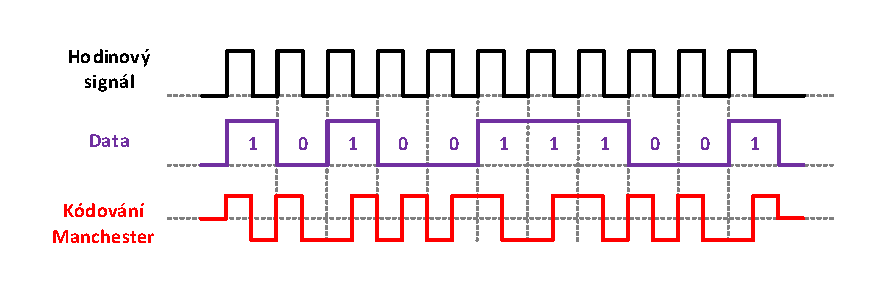
\includegraphics[scale=1.0]{obrazky/wmbus_manchester}
  \end{center}
	\vspace{-40pt}
  \caption{Princip kódování Manchester}
	\label{ObrazekManechester}
	\vspace{-10pt}
\end{figure}

Pokud nejsou vysílána žádná data, výstup kódování Manchester je hodinový signál. Nevýhodou použití Manchester kódování je to, že na přenos jednoho bitu informace je potřeba dvou hodinových taktů.

Princip kódování 3 ze 6 (viz Tab.~\ref{Table3out6}) spočívá v tom, že každé 4 bity (nibble) jsou zakódovány jako 6ti bitová data, přičemž zakódované slovo obsahuje stejné množství nul a jedniček. Zároveň v kódu musí být alespoň dvě změny, tzn. není možné použít \uv{000111} nebo \uv{111000}. Takto zakódovaná data jsou přenášené s nejvýznamnějším bitem jako prvním. Toto kódování by mělo být aplikováno při použití módu častého vysílání (módy T1 a T2) a při komunikaci měřiče s koncentrátorem. Koncentrátor může odpovědět měřiči zprávou kódovanou kódováním Manchester.


\begin{table}[!ht]
\centering
\caption{Tabulka kódování 3 ze 6 \cite{WMencodeing}}
\label{Table3out6}
\begin{tabular}{|c|c|c|c|c|}
\hline
\textbf{NRZ kód} & \textbf{Desítkově} & \textbf{3 ze 6} & \textbf{Desítkově} & \textbf{Počet změn v kódu} \\ \hline \hline
0                & 0                  & 10110               & 22                 & 4                          \\ \hline
1                & 1                  & 1101                & 13                 & 3                          \\ \hline
10               & 2                  & 1110                & 14                 & 2                          \\ \hline
11               & 3                  & 1011                & 11                 & 3                          \\ \hline
100              & 4                  & 11100               & 28                 & 2                          \\ \hline
101              & 5                  & 11001               & 25                 & 3                          \\ \hline
110              & 6                  & 11010               & 26                 & 4                          \\ \hline
111              & 7                  & 10011               & 19                 & 3                          \\ \hline
1000             & 8                  & 101100              & 44                 & 3                          \\ \hline
1001             & 9                  & 100101              & 37                 & 4                          \\ \hline
1010             & 10                 & 100110              & 38                 & 3                          \\ \hline
1011             & 11                 & 100011              & 35                 & 2                          \\ \hline
1100             & 12                 & 110100              & 52                 & 3                          \\ \hline
1101             & 13                 & 110001              & 49                 & 2                          \\ \hline
1110             & 14                 & 110010              & 50                 & 3                          \\ \hline
1111             & 15                 & 101001              & 41                 & 4                          \\ \hline \hline
\end{tabular}
\end{table}

\subsection{Linková vrstva Wireless M-Bus}

Linková vrstva poskytuje rozhraní mezi fyzickou a aplikační vrstvou. Její hlavní funkce jsou:
\begin{itemize}
	\item Poskytování služeb převádějících data mezi fyzickou a aplikační vrstvou.
	\item Generování CRC pro odchozí zprávy.
	\item Detekování CRC chyb v příchozích zprávách.
	\item Poskytování adresování fyzické vrstvy.
	\item Kontrola ACK u obousměrných přenosů.
	\item Vytváření rámců.
	\item Kontrola chyb rámců v příchozích zprávách.
\end{itemize}

Rámec linkové vrstvy se skládá z bloků dat. Každý blok dat obsahuje 16bitové CRC pole.  První blok má pevnou délku 12 bajtů a obsahuje L, C, M a A pole.

\subsubsection{L-Pole}
\begin{itemize}
	\item Určuje velikost přenášených dat, ale bez samotného L-pole a kontrolního součtu.	
\end{itemize}

\subsubsection{C-Pole}
\begin{itemize}
	\item Identifikuje typ rámce (SEND, CONFIRM, REQUEST, RESPONSE).
	\item Používá se pro zasílání základních příkazů.
\end{itemize}

\subsubsection{M-Pole}
\begin{itemize}
	\item Obsahuje identifikaci výrobce zařízení.
	\item Je kódováno jako třípísmenný kód, který se získává následovně:
			\begin{figure}[!ht]
				\begin{centerverbatim}
				Manufacturer ID = [ASCII(Znak1) - 64] + 32 + 32
												+ [ASCII(Znak2) - 64] + 32
												+ [ASCII(Znak3) - 64]
				\end{centerverbatim}
			\end{figure}
\end{itemize}
\vspace{-30pt}

\subsubsection{A-Pole}
\begin{itemize}
	\item Obsahuje 6 bajtů určující adresu zařízení.
	\item U rámců SEND a REQUEST je zde adresa vysílajícího zařízení.
	\item U rámců CONFIRM a RESPONSE je zde adresa zařízení, které je paket určen.
	\item Je tvořen následovně:
		\begin{itemize}
			\item 4 bajty (identifikační číslo) kódované jako 8 BCD znaků. Jedná se o unikátní identifikaci stanovenou výrobcem.
			\item 2 bajty (verze zařízení) určující generaci daného zařízení ve výrobním procesu výrobce.
			\item 2 bajty (typ zařízení), kódované dle Tab.~\ref{def_device_type_identification}.
		\end{itemize}
\end{itemize}

			\begin{table}[!ht]
			\centering
			\vspace{-10pt}
			\caption{Identifikace typu zařízení}
			\label{def_device_type_identification}
			\begin{tabular}{|c|c|c|c|c|c|}
			\hline
			\textbf{Hodnota} & \textbf{Bit 16}   & \textbf{Bit 15}   & \textbf{Bit 8}   & \textbf{Bit 7}  & \textbf{Médium  }                      \\ \hline\hline
			0           & 0        & 0        & 0       & 0      & Ostatní                   \\ \hline
			1           & 0        & 0        & 0       & 1      & Olej                     \\ \hline
			2           & 0        & 0        & 1       & 0      & Elektřina             \\ \hline
			3           & 0        & 0        & 1       & 1      & Benzín                     \\ \hline
			4           & 0        & 1        & 0       & 0      & Vytápění                    \\ \hline
			5           & 0        & 1        & 0       & 1      & Pára                   \\ \hline
			6           & 0        & 1        & 1       & 0      & Horká voda               \\ \hline
			7           & 0        & 1        & 1       & 1      & Voda                   \\ \hline
			8           & 1        & 0        & 0       & 0      & Tepelné čerpadlo                \\ \hline
			9           & 1        & 0        & 0       & 1      & Rezervováno                \\ \hline
			A           & 1        & 0        & 1       & 0      & Benzín 2              \\ \hline
			B           & 1        & 0        & 1       & 1      & Vytápění 2             \\ \hline
			C           & 1        & 1        & 0       & 0      & Horká voda 2        \\ \hline
			D           & 1        & 1        & 0       & 1      & Voda 2            \\ \hline
			E           & 1        & 1        & 1       & 0      & Tepelné čerpadlo 2           \\ \hline
			F           & 1        & 1        & 1       & 1      & Rezervováno                 \\ \hline\hline
			\end{tabular}
			\vspace{-5pt}
			\end{table}

\vspace{-10pt}
\subsubsection{CI-Pole}
\begin{itemize}
	\item Určuje typ přenášených dat.
	\item Nejčastější typy jsou uvedeny v Tab.~\ref{def_ci_pole}.
\end{itemize}

		\begin{table}[!ht]
		\centering
		\vspace{-30pt}
		\caption{Kódování CI-Pole}
		\label{def_ci_pole}
		\begin{tabular}{|c|c|c|}
\hline
\textbf{Hodnota} & \multicolumn{1}{c|}{\textbf{Direction}} & \multicolumn{1}{c|}{\textbf{Protokol}} \\ \hline \hline
50h               & Výběr aplikace zařízení           & pouze M-Bus    \\ \hline
51h               & Požadavek na zařízení                              & pouze M-Bus      \\ \hline
52h               & Výběr zařízení                    & pouze M-Bus      \\ \hline
5Ah               & Požadavek na zařízení                           & (W)M-Bus          \\ \hline
5Bh               & Požadavek na zařízení                            & M-Bus         \\ \hline
60h               & Požadavek na zařízení                            & DLMS         \\ \hline
61h               & Požadavek na zařízení                            & DLMS        \\ \hline
64h               & Požadavek na zařízení                            & SML     \\ \hline
65h               & Požadavek na zařízení                            & SML a   \\ \hline
6Ch               & Synchonizace času zařízení                     & všechny OMS     \\ \hline
6Dh               & Synchonizace času zařízení                       & všechny OMS        \\ \hline
6Eh               & Chyba zařízení                      & všechny OMS       \\ \hline
6Fh               & Chyba zařízení                        & všechny OMS       \\ \hline
70h               & Chyba zařízení                       & pouze M-Bus                    \\ \hline
71h               & Alarm zařízení                       & pouze M-Bus                    \\ \hline
72h               & Odpověd zařízení                     & (W)M-Bus                                              \\ \hline
74h               & Alarm zařízení                         & všechny OMS                                            \\ \hline
75h               & Alarm zařízení                         & všechny OMS                                            \\ \hline
78h               & Odpověd zařízení                   & (W)M-Bus                           \\ \hline
7Ah               & Odpověd zařízení                     & (W)M-Bus                                              \\ \hline
7Ch               & Odpověd zařízení                    & DLMS                                          \\ \hline
7Dh               & Odpověd zařízení                     & DLMS                                         \\ \hline
7Eh               & Odpověd zařízení                     & SML                                           \\ \hline
7Fh               & Odpověd zařízení                     & SML                                           \\ \hline \hline
\end{tabular}
\vspace{-10pt}
\end{table}

\subsubsection{CRC}
\begin{itemize}
	\item CRC obsahuje kontrolní součet pro kontrolu správnosti přenosu. 
	\item Jako kontrolní polynom se dle specifikace používá x\textsuperscript{16} + x\textsuperscript{13} + x\textsuperscript{12} + x\textsuperscript{11} + x\textsuperscript{10} + x\textsuperscript{8} +\textsuperscript{6} + x\textsuperscript{5} + x\textsuperscript{2} + 1.
\end{itemize}

\subsubsection{RSSI}
\begin{itemize}
	\item Received Signal Strength Indication.
	\item Určuje sílu signálu při přijetí paketu.
	\item Pro převod je využita lineární konverze:
\end{itemize}	
				\begin{figure}[!ht]
				\begin{centerverbatim}
				RSSI [dBm] = RSSI_LEVEL/2 - 130
				\end{centerverbatim}
			\end{figure}


%%%%%%%%%%%%%%%%%%%%%%%%%%%%%%%%%%%%%%%%%%%%%%%%%%%%%%%%%%%%%%%%%%%%%%%%%%%%%%%%%%%%%%%%%%
%%%%%%%%%%%%%%%%%%%%%%%%%%%%%%%%%%%%%%%%%%%%%%%%%%%%%%%%%%%%%%%%%%%%%%%%%%%%%%%%%%%%%%%%%%
%%%%%%%%%%%%%%%%%%%%%%%%%%%%%%%%%%%%%%%%%%%%%%%%%%%%%%%%%%%%%%%%%%%%%%%%%%%%%%%%%%%%%%%%%%
%%%%%%%%%%%%%%%%%%%%%%%%%%%%%%%%%%%%%%%%%%%%%%%%%%%%%%%%%%%%%%%%%%%%%%%%%%%%%%%%%%%%%%%%%%

\subsection{Aplikační vrstva Wireless M-Bus}

V souladu se specifikací OMS~(Open Metering Standard)~3.0.1~\cite{NormaOMS}, která vychází z normy EN 13757-4~\cite{Norma4} pro bezdrátový protokol WM-Bus, jsou některé položky aplikační vstvy shodné pro většinu zařízení protokolu WM-Bus.


\subsubsection{Access Number}
\begin{itemize}
	\item Binárně kódované pořadí přístupu.
	\item Při každém odeslání paketu je jeho hodnota zvýšena o jedničku.
	\item Po dosažení hodnoty 254 se začíná odznova.
\end{itemize}

\subsubsection{Status}
\begin{itemize}
	\item Obsahuje chyby vysílajícího zařízení.
	\item Může nastat i několik chyb zároveň.
	\item Definované chyby jsou uvedeny v Tab.~\ref{def_status}.
\end{itemize}

				\begin{table}[!ht]
				\centering
				\vspace{-10pt}
				\caption{Hodnoty Status pole}
				\label{def_status}
				\begin{tabular}{|c|c|l|}
				\hline
				\textbf{Bit}       & \textbf{Hex hodnota} & \textbf{Význam}        \\ \hline \hline
				\multirow{2}{*}{0} & 00h                  & Žádná chyba            \\ \cline{2-3} 
													 & 01h                  & Aplikace zaneprázdněna \\ \hline
				\multirow{2}{*}{1} & 02h                  & Obecná chyba aplikace  \\ \cline{2-3} 
													 & 03h                  & Neočekávaný stav       \\ \hline
				2                  & 04h                  & Vybitá baterie         \\ \hline
				3                  & 08h                  & Trvalá chyba           \\ \hline
				4                  & 10h                  & Dočasná chyba          \\ \hline
				5                  & 20h                  & Specifický kód výrobce \\ \hline
				6                  & 40h                  & Specifický kód výrobce \\ \hline
				7                  & 80h                  & Specifický kód výrobce \\ \hline \hline
				\end{tabular}
				\end{table}


Struktura zbytku aplikační vrstvy je dána opakováním určité sekvence (viz Tab.~\ref{TableStrukturaDat}) bajtů, určující typ a hodnotu přenášených dat.
\begin{table}[!ht]
\centering
\caption{Struktura dat aplikační vrstvy}
\label{TableStrukturaDat}
\begin{tabular}{|c|c|c|c|c|}
\hline
\textbf{Byte 1}                                                                & \textbf{Byte 2}                                                                             & \textbf{Byte 3}                                                                & \textbf{Byte 4}                                                                             & \textbf{Byte 5-n}                                                      \\ \hline \hline
\multicolumn{2}{|c|}{\begin{tabular}[c]{@{}c@{}}Data Information \\ Block (DIB)\end{tabular}}                                                                                & \multicolumn{2}{c|}{\begin{tabular}[c]{@{}c@{}}Value Information \\ Block (VIB)\end{tabular}}                                                                                & \multirow{2}{*}{\begin{tabular}[c]{@{}c@{}}Data\\ Values\end{tabular}} \\ \cline{1-4}
\begin{tabular}[c]{@{}c@{}}Data  \\ Information \\ Field\\  (DIF)\end{tabular} & \begin{tabular}[c]{@{}c@{}}Data \\ Information \\ Field \\ Extension \\ (DIFE)\end{tabular} & \begin{tabular}[c]{@{}c@{}}Value \\ Information \\ Field \\ (VIF)\end{tabular} & \begin{tabular}[c]{@{}c@{}}Data \\ Information \\ Field \\ Extension \\ (VIFE)\end{tabular} &                                                                        \\ \hline \hline
\end{tabular}
\end{table}

\vspace{-10pt}
\subsubsection{Data Information Block (DIB)}
DIB definuje typ přenášených dat a skládá se z DIF a z nepovinného DIFE.

\subsubsection{Data information Field (DIF)}
DIF definuje datový typ přenášených dat a má strukturu dle Tab.~\ref{KodovaniDIFu}.
	\begin{table}[!ht]
	\centering
	\caption{Kódování DIF Pole}
	\label{KodovaniDIFu}
	\begin{tabular}{|c|c|c|c|c|c|c|c|}
	\hline \hline
	\textbf{Bit 1}                                           & \textbf{Bit2}                                                    & \textbf{Bit 3}                         & \textbf{Bit 4}                        & \textbf{Bit 5} & \textbf{Bit 6} & \textbf{Bit 7} & \textbf{Bit 8} \\ \hline 
	\begin{tabular}[c]{@{}c@{}}Rozšiřující \\ Bit\end{tabular} & \begin{tabular}[c]{@{}c@{}}LSB uložení\end{tabular} & \multicolumn{2}{c|}{\begin{tabular}[c]{@{}c@{}}Funkční \\ Položka\end{tabular}} & \multicolumn{4}{c|}{Data}                                         \\ \hline \hline
	\end{tabular}
	\end{table}

Rozšiřující bit pole určuje jaký blok bajtů následuje po DIF. Možnosti jsou shrnuty v Tab.~\ref{KodovaniRozsBituDIFu}.

\begin{table}[!ht]
\centering
\caption{Kódování rozšiřujícího bitu DIF pole}
\label{KodovaniRozsBituDIFu}
\begin{tabular}{|c|c|}
\hline
\textbf{Bit} & \textbf{Další informace je obsažena v} \\ \hline \hline
0            & DIF                                    \\ \hline
1            & DIFE                                   \\ \hline \hline
\end{tabular}
\end{table}

Funkční pole definuje typ přenášené hodnoty z hlediska její aktuálnosti či limitnosti. Možnosti jsou shrnuty v Tab.~\ref{KodovaniFunkPoleDIFu}.

\begin{table}[!ht]
\centering
\caption{Kódování funkčního pole DIF pole}
\label{KodovaniFunkPoleDIFu}
\begin{tabular}{|c|l|}
\hline
\textbf{Hodnota} & \multicolumn{1}{c|}{\textbf{Význam}} \\ \hline \hline
00b              & Okamžitá hodnota                     \\ \hline
01b              & Minimální hodnota                    \\ \hline
10b              & Maximální hodnota                    \\ \hline
11b              & Hodnota při chybovém stavu         \\ \hline \hline
\end{tabular}
\end{table}

Data pole určuje datový typ přenášené hodnoty. Možnosti jsou shrnuty v Tab.~\ref{KodovaniDataPoleDIFu}.

\begin{table}[!ht]
\centering
\caption{Kódování Data pole DIF pole}
\label{KodovaniDataPoleDIFu}
\begin{tabular}{|c|c|c|c|c|}
\hline
\textbf{Délka hodnoty {[}b{]}} & \textbf{Kód} & \textbf{Význam} & \textbf{Kód} & \textbf{Význam}   \\ \hline \hline
0                              & 0000         & Žádná data      & 1000         & Volba pro hodnotu \\ \hline
8                              & 0001         & 8-bit Integer   & 1001         & 2 cifry BCD       \\ \hline
16                             & 0010         & 16-bit Integer  & 1010         & 4 cifry BCD       \\ \hline
24                             & 0011         & 24-bit Integer  & 1011         & 6 cifer BCD       \\ \hline
32                             & 0100         & 32-bit Integer  & 1100         & 8 cifer BCD       \\ \hline
32                             & 0101         & 32-bit Real     & 1101         & Proměnlivá délka  \\ \hline \hline
\end{tabular}
\end{table}

\subsubsection{Data Information Field Extension (DIFE)}
DIFE obsahuje upřesnění veličiny či informace o tarifu dle struktury zobrazené v Tab.~\ref{KodovaniDIFE}.

\begin{table}[!ht]
\centering
\caption{Kódování DIFE Pole}
\label{KodovaniDIFE}
\begin{tabular}{|c|c|c|c|c|c|c|c|}
\hline \hline
\textbf{Bit 7}  & \textbf{Bit 6} & \textbf{Bit 5} & \textbf{Bit 4} & \textbf{Bit 3} & \textbf{Bit 2} & \textbf{Bit 1} & \textbf{Bit 0} \\ \hline 
Rozšiřující bit & Jednotka       & \multicolumn{2}{c|}{Tarif}      & \multicolumn{4}{c|}{Hodnota}                                      \\ \hline \hline
\end{tabular}
\end{table}

\subsubsection{Value Information Block (VIB)}
VIB definuje typ přenášené hodnoty a skládá se z VIF a z nepovinného VIFE.

\subsubsection{Value Information Field (VIF)}
VIF definuje veličinu přenášených dat a má strukturu dle Tab.~\ref{KodovaniVIFu}.

\begin{table}[!ht]
\centering
\caption{Kódování VIF Pole}
\label{KodovaniVIFu}
\begin{tabular}{|c|c|c|c|c|c|c|c|}
\hline \hline
\textbf{Bit 1}  & \textbf{Bit2} & \textbf{Bit 3} & \textbf{Bit 4} & \textbf{Bit 5} & \textbf{Bit 6} & \textbf{Bit 7} & \textbf{Bit 8} \\ \hline 
Rozšiřující bit & \multicolumn{7}{c|}{Data}                                                                                           \\ \hline \hline
\end{tabular}
\end{table}

Rozšiřující bit pole určuje jaký blok bajtů následuje po VIF. Možnosti jsou shrnuty v Tab.~\ref{KodovaniRozsBituVIFu}.

\begin{table}[!ht]
\centering
\caption{Kódování rozšiřujícího bitu VIF pole}
\label{KodovaniRozsBituVIFu}
\begin{tabular}{|c|c|}
\hline
\textbf{Bit} & \textbf{Další informace je obsažena v} \\ \hline \hline
0            & VIF                                    \\ \hline
1            & VIFE                                   \\ \hline \hline
\end{tabular}
\end{table}

Data pole určuje datový typ přenášené hodnoty. Možnosti jsou shrnuty v Tab.~\ref{KodovaniDataPoleVIFu}.

\begin{table}[!ht]
\centering
\caption{Kódování Data pole VIF pole}
\label{KodovaniDataPoleVIFu}
\resizebox{\textwidth}{!}{%
\begin{tabular}{|l|l|l|l|}
\hline
\multicolumn{1}{|c|}{\textbf{Bity}} & \multicolumn{1}{c|}{\textbf{Veličina}} & \multicolumn{1}{c|}{\textbf{Jednotka}}                                                                                & \multicolumn{1}{c|}{\textbf{Rozsah}} \\ \hline \hline
E000 0nnn                             & Energie                                    & 10\textsuperscript{(nnn-3)}\,Wh                                                                                                              & 0.001\,Wh - 10000\,Wh \\ \hline
E000 1nnn                             & Energie                                    & 10\textsuperscript{(nnn)}\,J                                                                                                                 & 0.001\,kJ - 10000 \,kJ                \\ \hline
E001 0nnn                             & Objem                                    & 10\textsuperscript{(nnn-6)}\,m\textsuperscript{3}                                                                                                              & 0.001\,l - 10000\,l                    \\ \hline
E001 1nnn                             & Hmotnost                                      & 10\textsuperscript{(nnn-3)}\,kg                                                                                                              & 0.001\,kg - 10000\,kg                \\ \hline
\multirow{2}{*}{E010 00nn}            & \multirow{2}{*}{Provozní čas}                  & \multirow{4}{*}{\begin{tabular}[c]{@{}l@{}}nn = 00 sekundy\\ nn = 01 minuty\\ nn = 10 hodiny\\ nn = 11 dny\end{tabular}} & \multirow{2}{*}{}                   \\
                                      &                                           &                                                                                                                           &                                     \\ \cline{1-2} \cline{4-4} 
\multirow{2}{*}{E010 01nn}            & \multirow{2}{*}{Operační čas}            &                                                                                                                           & \multirow{2}{*}{}                   \\
                                      &                                           &                                                                                                                           &                                     \\ \hline
E010 1nnn                             & Výkon                                     & 10\textsuperscript{(nnn-3)}\,W                                                                                                               & 0.001\,W - 10000\,W                  \\ \hline
E011 0nnn                             & Výkon                                     & 10\textsuperscript{(nnn)}\,J/h                                                                                                               & 0.001\,kJ/h - 10000\,kJ/h            \\ \hline
E011 1nnn                             & Průtok                              & 10\textsuperscript{(nnn-6)}\,m\textsuperscript{3}/h                                                                                                            & 0.001\,l/h - 10000 l/h              \\ \hline
E100 0nnn                             & Průtok                           & 10\textsuperscript{(nnn-7)}\,m\textsuperscript{3}/min                                                                                                          & 0.0001\,l/min - 1000 l/min          \\ \hline
E100 1nnn                             & Průtok                           & 10\textsuperscript{(nnn-9)}\,m\textsuperscript{3}/s                                                                                                            & 0.001\,ml/s - 10000 ml/s            \\ \hline
E101 0nnn                             & Protok (hmotnosti)                              & 10\textsuperscript{(nnn-3)} kg/h                                                                                                            & 0.001\,kg/h - 10000 kg/h            \\ \hline
E101 10nn                             & Teplota (průtoku)                           & 10\textsuperscript{(nn-3)}\,°C                                                                                                               & 0.001\,°C - 1\,°C                    \\ \hline
E101 11nn                             & Teplota (návratová)                         & 10\textsuperscript{(nn-3)}\,°C                                                                                                               & 0.001\,°C - 1\,°C                    \\ \hline
E110 00nn                             & Teplota (rozdíl)                    & 10\textsuperscript{(nn-3)}\,K                                                                                                                & 1\,mK - 1000\,mK                     \\ \hline
E110 01nn                             & Temperature (externí)                       & 10\textsuperscript{(nn-3)}\,°C                                                                                                               & 0.001\,°C - 1\,°C                    \\ \hline
E110 10nn                             & Tlak                                 & 10\textsuperscript{(nn-3)}\,bar                                                                                                              & 1\,mbar - 1000\,mbar                 \\ \hline
\multirow{2}{*}{E110 110n}                             & \multirow{2}{*}{Datum a čas}                                & \multirow{2}{*}{\begin{tabular}[c]{@{}l@{}}n = 0 datum\\ n = 1 datum a čas\end{tabular}}                                                                                            & \multirow{2}{*}{Datový typ F a G}             \\ 
                                      &                                           &                                                                                                                           &                                     \\ \hline
E110 1110                             & Tepelná výměna                          &                                                                                                                           & bezrozměrné                 \\ \hline
E110 1111                             & Rezervováno                                 &                                                                                                                           &                                     \\ \hline
\multirow{2}{*}{E111 00nn}            & \multirow{2}{*}{Průměrné trvání}        & \multirow{4}{*}{\begin{tabular}[c]{@{}l@{}}nn = 00 sekundy\\ nn = 01 minuty\\ nn = 10 hodiny\\ nn = 11 dny\end{tabular}} & \multirow{2}{*}{}                   \\
                                      &                                           &                                                                                                                           &                                     \\ \cline{1-2} \cline{4-4} 
\multirow{2}{*}{E111 01nn}            & \multirow{2}{*}{Aktuální trvání}        &                                                                                                                           & \multirow{2}{*}{}                   \\
                                      &                                           &                                                                                                                           &                                     \\ \hline
E111 1000                             & Výrobní číslo                            &                                                                                                                           &                 \\ \hline
E111 1001                             & Rozšířená identifikace                &                                                                                                                           & Datový typ C                    \\ \hline
E111 1010                             & Adresa sběrnice                               &                                                                                                                           & Datový typ C                    \\ \hline \hline
\end{tabular}}
\end{table}

\subsubsection{Value Information Field Extension (VIFE)}
VIFE obsahují upřesnění, doplňující informaci či přenos chybového stavu dané položky. Jejich kompletní přehled je uveden ve specifikaci~\cite{WmBusSpecka}.

\begin{table}[!ht]
\centering
\caption{Kódování VIFE Pole}
\label{KodovaniVIFE}
\begin{tabular}{|c|c|c|c|c|c|c|c|}
\hline \hline
\textbf{Bit 7}  & \textbf{Bit 6} & \textbf{Bit 5} & \textbf{Bit 4} & \textbf{Bit 3} & \textbf{Bit 2} & \textbf{Bit 1} & \textbf{Bit 0} \\ \hline 
Rozšiřující bit & Jednotka       & \multicolumn{2}{c|}{Tarif}      & \multicolumn{4}{c|}{Hodnota}                                      \\ \hline \hline
\end{tabular}
\end{table}

\subsubsection{Data Value}
Pole \texttt{Data Value} již obsahuje přenášenou hodnotu, definovanou dle DIB a VIB.


\subsubsection{Datové typy F a G}
V protokolu Wireless M-Bus je datum kódováno ve formátu G, viz Tab.~\ref{KodovaniDataG} 

\begin{table}[!ht]
\centering
\caption{Kódování data ve formátu G}
\label{KodovaniDataG}
\begin{tabular}{|c|c|c|c|c|c|c|c|c|c|c|c|c|c|c|c|}
\hline
\rotatebox[origin=c]{90}{\parbox[b]{1.75cm}{\hspace{10pt}\textbf{Bit 7}}} & 
\rotatebox[origin=c]{90}{\parbox[b]{1.75cm}{\hspace{10pt}\textbf{Bit 6}}} & 
\rotatebox[origin=c]{90}{\parbox[b]{1.75cm}{\hspace{10pt}\textbf{Bit 5}}} &
\rotatebox[origin=c]{90}{\parbox[b]{1.75cm}{\hspace{10pt}\textbf{Bit 4}}} & 
\rotatebox[origin=c]{90}{\parbox[b]{1.75cm}{\hspace{10pt}\textbf{Bit 3}}} & 
\rotatebox[origin=c]{90}{\parbox[b]{1.75cm}{\hspace{10pt}\textbf{Bit 2}}} &
\rotatebox[origin=c]{90}{\parbox[b]{1.75cm}{\hspace{10pt}\textbf{Bit 1}}} & 
\rotatebox[origin=c]{90}{\parbox[b]{1.75cm}{\hspace{10pt}\textbf{Bit 0}}} & 
\rotatebox[origin=c]{90}{\parbox[b]{1.75cm}{\hspace{10pt}\textbf{Bit 7}}} &
\rotatebox[origin=c]{90}{\parbox[b]{1.75cm}{\hspace{10pt}\textbf{Bit 6}}} & 
\rotatebox[origin=c]{90}{\parbox[b]{1.75cm}{\hspace{10pt}\textbf{Bit 5}}} & 
\rotatebox[origin=c]{90}{\parbox[b]{1.75cm}{\hspace{10pt}\textbf{Bit 4}}} &
\rotatebox[origin=c]{90}{\parbox[b]{1.75cm}{\hspace{10pt}\textbf{Bit 3}}} & 
\rotatebox[origin=c]{90}{\parbox[b]{1.75cm}{\hspace{10pt}\textbf{Bit 2}}} & 
\rotatebox[origin=c]{90}{\parbox[b]{1.75cm}{\hspace{10pt}\textbf{Bit 1}}} &
\rotatebox[origin=c]{90}{\parbox[b]{1.75cm}{\hspace{10pt}\textbf{Bit 0}}} \\ \hline \hline
\multicolumn{8}{|c|}{Bajt 1} & \multicolumn{8}{c|}{Bajt 2} \\ \hline
\multicolumn{3}{|c|}{Rok (1/2)} & \multicolumn{5}{c|}{Den} & \multicolumn{4}{c|}{Rok (2/2)} & \multicolumn{4}{c|}{Měsíc} \\ \hline \hline
\end{tabular}
\end{table}

a datum i čas ve formátu F, viz Tab.~\ref{KodovaniDataF}.  

\begin{table}[!ht]
\centering
\caption{Kódování data a času ve formátu F}
\label{KodovaniDataF}
\begin{tabular}{|c|c|c|c|c|c|c|c|c|c|c|c|c|c|c|c|c|c|}
\hline
\rotatebox[origin=c]{90}{\parbox[b]{1.75cm}{\hspace{10pt}\textbf{Bit 7}}} & 
\rotatebox[origin=c]{90}{\parbox[b]{1.75cm}{\hspace{10pt}\textbf{Bit 6}}} & 
\rotatebox[origin=c]{90}{\parbox[b]{1.75cm}{\hspace{10pt}\textbf{Bit 5}}} &
\rotatebox[origin=c]{90}{\parbox[b]{1.75cm}{\hspace{10pt}\textbf{Bit 4}}} & 
\rotatebox[origin=c]{90}{\parbox[b]{1.75cm}{\hspace{10pt}\textbf{Bit 3}}} & 
\rotatebox[origin=c]{90}{\parbox[b]{1.75cm}{\hspace{10pt}\textbf{Bit 2}}} &
\rotatebox[origin=c]{90}{\parbox[b]{1.75cm}{\hspace{10pt}\textbf{Bit 1}}} & 
\rotatebox[origin=c]{90}{\parbox[b]{1.75cm}{\hspace{10pt}\textbf{Bit 0}}} & 
\rotatebox[origin=c]{90}{\parbox[b]{1.75cm}{\hspace{10pt}\textbf{Bit 7}}} &
\rotatebox[origin=c]{90}{\parbox[b]{1.75cm}{\hspace{10pt}\textbf{Bit 6}}} & 
\rotatebox[origin=c]{90}{\parbox[b]{1.75cm}{\hspace{10pt}\textbf{Bit 5}}} & 
\rotatebox[origin=c]{90}{\parbox[b]{1.75cm}{\hspace{10pt}\textbf{Bit 4}}} &
\rotatebox[origin=c]{90}{\parbox[b]{1.75cm}{\hspace{10pt}\textbf{Bit 3}}} & 
\rotatebox[origin=c]{90}{\parbox[b]{1.75cm}{\hspace{10pt}\textbf{Bit 2}}} & 
\rotatebox[origin=c]{90}{\parbox[b]{1.75cm}{\hspace{10pt}\textbf{Bit 1}}} &
\rotatebox[origin=c]{90}{\parbox[b]{1.75cm}{\hspace{10pt}\textbf{Bit 0}}} & & \\ \hline \hline
\multicolumn{8}{|c|}{Bajt 1}                                  & \multicolumn{8}{c|}{Bajt 2}                                   & Bajt 3           & Bajt 4          \\ \hline
0     & 0     & \multicolumn{6}{c|}{Hodina}                   & 0     & 0     & 0     & \multicolumn{5}{c|}{Minuta}           & \multicolumn{2}{c|}{Dle formátu G} \\ \hline \hline
\end{tabular}
\end{table}

Ukázky implementace obou formátů v jazyce Python uvádí Kód~\ref{CodeFG}.

\begin{lstlisting}[caption={Implementace F a G formátu},captionpos=b,label=CodeFG,style=MyCodePython]
# Get date in G format
def get_date(date_bytes):
    date = str(bin(int(date_bytes[0:2], 16))[2:]).zfill(8) + str(bin(int(date_bytes[2:4], 16))[2:]).zfill(8)
    year = str(int(date[0:4] + date[8:11], 2))
    month = str(int(date[4:8], 2))
    day = str(int(date[11:16], 2))
    vysledek = day + "." + month + ".20" + year
    return vysledek

# Get time from F format
def get_time(time_bytes):
    time = str(bin(int(time_bytes[0:2], 16))[2:]).zfill(8) + str(bin(int(time_bytes[2:4], 16))[2:]).zfill(8)
    hour = str(int(time[3:8], 2))
    minute = str(int(time[10:16], 2)).zfill(2)
    vysledek = hour + ":" + minute
    return vysledek
\end{lstlisting}
	
\newpage{}	
	
\section{Šifrování dat}
Pro šifrování přenášených dat se v protokolu Wireless M-Bus používají tři šifrovací algoritmy:
\begin{itemize}
	\item DES (Data Encryption Standard) bez inicializačního vektoru,
	\item DES s inicializačním vektorem a
	\item AES (Advanced Encryption Standard) s inicializačním vektorem.
\end{itemize}

Šifrování DES dnes již není moc využívané, je již nedostačující a zastaralé. Drtivá většina dnešních zařízení umožnujících šifrovaný přenos využívají šifrování AES, konkrétně verzi AES128 CBC.

\subsection{Šifrovací algoritmus DES}
Data Encryption Standard je v kryptografii symetrická šifra vyvinutá v 70. letech. V roce 1977 byla zvolena za standard FIPS 46~\cite{NormaFIPS46}. V současnosti je tato šifra považována za nespolehlivou, protože používá klíč pouze o délce 64 bitů, z toho 8 je kontrolních a 56 efektivních. Navíc algoritmus obsahuje slabiny, které dále snižují bezpečnost šifry. Díky tomu je možné šifru prolomit útokem hrubou silou za méně než 24 hodin.

\subsection{Šifrovací algoritmus AES}
Advanced Encryption Standard je symetrická bloková šifra (pro šifrování i dešifrování využívá stejný klíč na data s pevně danou délkou bloku), která nahradila dříve užívanou šifru DES~\cite{NormaFIPS}. AES šifra je rychlá v softwaru i hardwaru a na rozdíl od~svého předchůdce DES nepoužívá Feistelovu síť. AES má pevně danou velikost bloku na 128 bitů a velikost klíče na 128, 192 nebo 256 bitů.   Pokud jsou šifrovaná data delší, zpracovávají se po jednotlivých blocích. 

\begin{figure}[!ht]
\vspace{-10pt}
 \begin{center}
    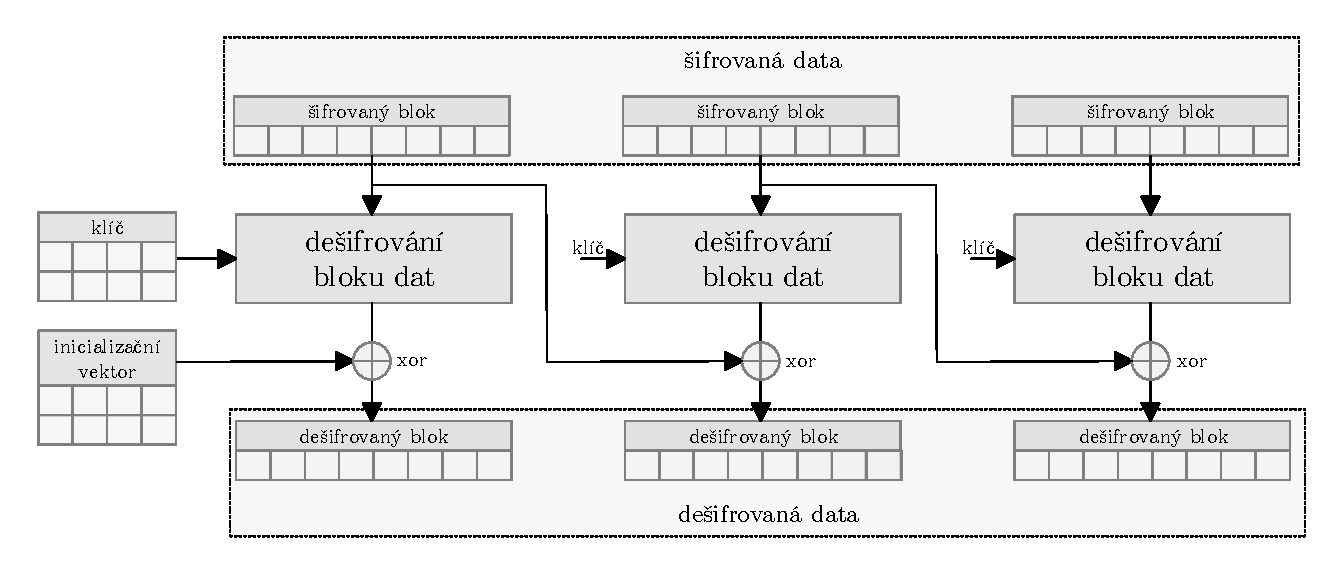
\includegraphics[scale=0.65]{obrazky/wmbus_aes_cbc}
  \end{center}
	\vspace{-30pt}
  \caption{Princip algoritmu AES v módu CBC}
	\label{SchemaAEScbc}
	\vspace{-10pt}
\end{figure}

Pro šifrovaný přenos dat v protokolu WM-Bus se využívá AES, kontrétně mód s~inicializačním vektorem (CBC - Cipher Block Chaining). Ten funguje (viz~Obr.~\ref{SchemaAEScbc}) tak, že před zašifrováním se odpovídající blok otevřeného textu xoruje předcházejícím blokem zašifrovaného textu. To znamená, že jednotlivé bloky jsou na sobě závislé, aby došlo k dešifrování konkrétního bloku, je nutné  dešifrovat i všechny předchozí. Je tedy nutné mít nějaký nulový blok dat pro zašifrování prvního bloku dat. K tomu se využívá inicializační vektor. Tomuto bloku se pak říká inicializační vektor (IV). Tento blok se použije k dešifrování prvního bloku a pak zahodí.



\subsection{Inicializační vektor}
\label{KapitolaInicializacniVektor}
Inicializační vektor má délku 16 Bajtů (128 bitů, odtud označení AES-128) a~v~případě protokolu WM-Bus je tvořený dynamicky z nešifrovaných bajtů polí paketu, způsobem popsaným v Tab.~\ref{TabulkaInicializacniVektor} a implemetovaných dle Kódu~\ref{CodeIV}.

\begin{lstlisting}[caption={Sestavení inicializačního vektoru},captionpos=b,label=CodeIV,style=MyCodePython]
# Build Initialization Vector from incoming packet data
device = parsedstring[8:24].upper()
access = str(parsedstring[26:28])
AES_IV = binascii.unhexlify(device + access * 8)
\end{lstlisting}

\begin{table}[!ht]
	%\vspace{-30pt}
  \caption{Formát inicializačního vektoru}
	\label{TabulkaInicializacniVektor}
	\vspace{-10pt}
	\begin{center}
\begin{tabular}{|c|c|l|}
\hline
\textbf{Bit} & \textbf{Obsah}                 & \textbf{Význam}                        \\ \hline \hline
LSB          & \multirow{2}{*}{M-Pole}        & \multirow{2}{*}{Identifikace výrobce}  \\ \cline{1-1}
1            &                                &                                        \\ \hline
2            & \multirow{6}{*}{A-Pole}        & \multirow{6}{*}{Identifikace zařízení} \\ \cline{1-1}
3            &                                &                                        \\ \cline{1-1}
4            &                                &                                        \\ \cline{1-1}
5            &                                &                                        \\ \cline{1-1}
6            &                                &                                        \\ \cline{1-1}
7            &                                &                                        \\ \hline
8            & \multirow{2}{*}{Access Number} & \multirow{8}{*}{Identifikace paketu}   \\ \cline{1-1}
9            &                                &                                        \\ \cline{1-2}
10           & \multirow{2}{*}{Access Number} &                                        \\ \cline{1-1}
11           &                                &                                        \\ \cline{1-2}
12           & \multirow{2}{*}{Access Number} &                                        \\ \cline{1-1}
13           &                                &                                        \\ \cline{1-2}
14           & \multirow{2}{*}{Access Number} &                                        \\ \cline{1-1}
MSB          &                                &                                        \\ \hline \hline
\end{tabular}
\vspace{-20pt}
\end{center}
\end{table}

První 2 bajty obsahují přidělené identifikační údaje výrobce, další čtyři obsahují sériové číslo daného zařízení, následující dva obsahují verzi zařízení a zbylých osm Bajtů je tvořeno opakováním se přístupového čísla. Vzhledem k faktu, že přístupové číslo se s každým vysláním telegramu změní, je nutné inicializační vektor přepočítat pro každý přijatý paket. Tím je zajištěna dynamičnost šifrování danou metodou.

\subsection{Šifrovací klíč}
Šifrovací klíč AES je sekvence bajtů o velikosti 128, 192 nebo 256 bitů. Tento klíč slouží pro šifrování a dešifrování přenášených dat a je unikátní pro každé vyčítané zařízení. Bez znalosti tohoto klíče nelze tedy vyčítat zařízení se šifrovaným přenosem dat.

\newpage{}

\subsection{Určení šifrovaných dat}
\label{KapitolaConfigurationWord}
Aplikační vrstva protokolu WM-Bus obsahuje položku \texttt{ConfigurationWord} případně \texttt{SignatureField}, která deklaruje typ použitého šifrovací algoritmu, délku šifrované části a způsob datového šifrování. Pole je složeno ze dvou bajtů. První bajt obsahuje \texttt{NNNNCCHHb} a druhý bajt obsahuje \texttt{BAS0MMMMb}. Význam jednotlivých položek je shrnut v Tab.~\ref{TableConfigurationWord}.


\begin{table}[!ht]
\centering
\caption{Význam bitů pole ConfigurationWord}
\label{TableConfigurationWord}
\begin{tabular}{|c|c|l|}
\hline
\textbf{Bit} & \textbf{Označení} & \textbf{Význam}        \\ \hline \hline
MSB          & B                 & Obousměrnost           \\ \hline
14           & A                 & Dostupnost             \\ \hline
13           & S                 & Synchronizace          \\ \hline
12           & 0                 & Synchronizace          \\ \hline
11           & M                 & Šifrování              \\ \hline
10           & M                 & Šifrování              \\ \hline
9            & M                 & Šifrování              \\ \hline
8            & M                 & Šifrování              \\ \hline
7            & N                 & Počet kódovaných bloků \\ \hline
6            & N                 & Počet kódovaných bloků \\ \hline
5            & N                 & Počet kódovaných bloků \\ \hline
4            & N                 & Počet kódovaných bloků \\ \hline
3            & C                 & Obsah telegramu        \\ \hline
2            & C                 & Obsah telegramu        \\ \hline
1            & H                 & Počítač skoků          \\ \hline
LSB          & H                 & Počítač skoků          \\  \hline  \hline
\end{tabular}
%\vspace{-5pt}
\end{table}

Bity šifrování nabývají těchto hodnot:
\begin{itemize}
	\item 4 pro AES se statickým inicializačním vektorem,
	\item 5 pro AES s dynamickým inicializačním vektorem,
	\item 6 je rezervovaná,
	\item 7 až 15 jsou pro využití výrobcem.
\end{itemize}
Pro režim AES s dynamickým inicializačním vektorem bity jsou 0101 a vyjadřují hodnotu 5.

\newpage{}

\subsection{Princip dešifrování}
Pro dešifrování přijatých dat je nutná znalost šifrovacího algoritmu, šifrovacího klíče a sestavení inicializačního vektoru. Potom lze aplikací dešifrovacího algoritmu získat přenášená data. Obecné schéma dešifrování AES-128 CBC je znázorněno na~Obr.~\ref{SchemaAESobecne} a~implementováno v~Kódu~\ref{CodeCrypto}.
\begin{figure}[!ht]
\vspace{-20pt}
 \begin{center}
    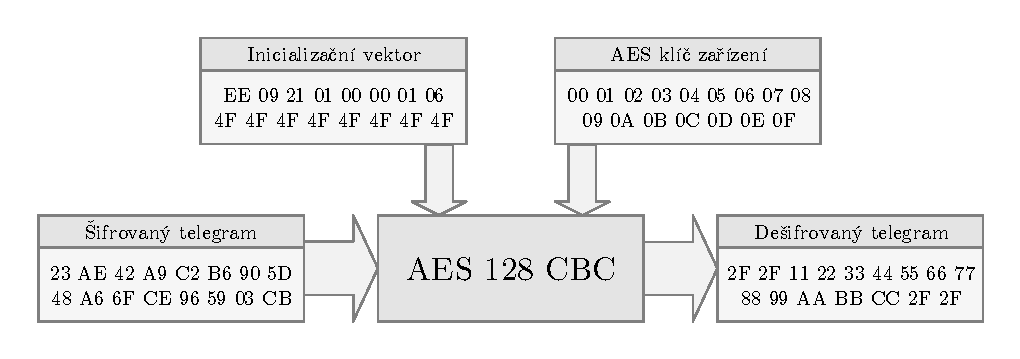
\includegraphics[scale=0.8]{obrazky/wmbus_aes_schema}
  \end{center}
	\vspace{-30pt}
  \caption{Obecné schéma dešifrování AES-128 CBC}
	\label{SchemaAESobecne}
	\vspace{-20pt}
\end{figure}

\begin{lstlisting}[caption={Implementace AES},captionpos=b,label=CodeCrypto,style=MyCodePython]
from Crypto.Cipher import AES

encryptor = AES.new(AES_KEY_IQRF, AES.MODE_CBC, IV=AES_IV)
OUTPUT_DECRYPTED = encryptor.decrypt(INPUT_ENCRYPTED)
\end{lstlisting}

\subsection{Kontrola rozšifrování dat}
Ke kontrole správnosti dešifrovaných dat slouží definovaná počáteční sekvence dat. U algoritmu DES začínají dešifrovaná data dvěma bajty obsahujícími datum a čas. Pro algoritmus AES jsou první dva bajty šestnáckové a oba obsahují znak 2Fh, jak znázorňuje Kód~\ref{CodeVerify}.

\begin{lstlisting}[caption={Ověření kontrolní sekvence AES},captionpos=b,label=CodeVerify,style=MyCodePython]
# Verify control sequence after decrypt
aes_control = binascii.hexlify(TELEGRAM_ORIGINAL[0:2]).upper()
if (aes_control == b'2F2F'):
		binascii.hexlify(TELEGRAM_ORIGINAL).upper().decode('ascii'))
\end{lstlisting}

